\section{Case Studies on Public Datasets}
\label{sec:case}

To test the argument of \cref{sec:egonoise} rather than assert it, we run three reproducible studies with established methods and one shared code base, on three public datasets.
\Cref{sec:case-dregon} measures how much an explicit noise model and motor-speed information help in-flight localization on one drone.
\Cref{sec:case-drones} asks whether the properties of ego-noise that make such models work hold across five different drones.
\Cref{sec:case-locata} applies the same localizers to a robot-head array in a reverberant room without ego-noise, to see where a noise model stops helping.
The code reproduces every number and figure in this section.

\subsection{In-flight localization on a drone (DREGON)}
\label{sec:case-dregon}

DREGON~\cite{strauss2018dregon} records an 8-microphone array on a quadrotor, together with each rotor's measured speed (logged at about 1\,kHz), the flight controller's IMU and the true source direction from motion capture.
We use the noise-only flight to learn noise models, two free flights with a white-noise loudspeaker (391 windows of 0.5\,s) for evaluation, and the clean tripod recordings mixed with held-out flight noise for a controlled SNR sweep.

\paragraph{Setup.}
We compare five localizers on a $3^\circ$ grid and a 300--4000\,Hz band: (A) SRP-PHAT~\cite{dibiase2000srp}; (B) SRP-PHAT with bins at predicted rotor harmonics removed, using the motor log; (C) MUSIC~\cite{schmidt1986music}; (D) GEVD-MUSIC (\cref{eq:gevd}) with a single noise covariance learned from the noise-only flight~\cite{nakamura2011gevd,furukawa2013ncm}; and (E) GEVD-MUSIC with six covariances binned by mean motor speed, a simple form of state-informed modeling~\cite{furukawa2013ncm,yen2023ncm}.
The array and motion-capture frames are aligned once, with method A only, on a separate flight with motors off (median error after alignment $2.5^\circ$).
The motor-speed unit is not documented by the dataset; aligning predicted rotor harmonics with the noise spectrum shows that the logged values are revolutions per second (best-fitting scale 0.997).

\paragraph{Localization in flight.}
\Cref{tab:case} gives the headline numbers.
Without a noise model (A, C) most windows are wrong by tens of degrees: the response peaks in the directions of the rotors, about $45^\circ$ above the array.
Learning the noise covariance (D) reduces the median error from $77^\circ$ to $6^\circ$, and selecting it by motor speed (E) adds a further 9 points of accuracy.
The benefit of motor speed is concentrated on the harder, quieter-source flight, where E reaches 64\% within $10^\circ$ against 47\% for D, and the median error falls from $31^\circ$ to $5^\circ$.
Masking predicted rotor tones (B) helps the baseline but cannot rescue it, because much of the rotor noise is broadband.
\Cref{fig:tracking} shows the difference over whole flights.

\begin{table}[t]
\centering
\footnotesize
\setlength{\tabcolsep}{2.4pt}
\begin{tabular}{@{}lcccc@{}}
\toprule
 & \multicolumn{2}{c}{Both flights} & \multicolumn{2}{c}{Within $10^\circ$} \\
\cmidrule(lr){2-3}\cmidrule(l){4-5}
Method & Med. err. & ${\le}10^\circ$ & Loud & Quiet \\
\midrule
A\; SRP-PHAT & $76.7^\circ$ & 18.4\% & 36.1\% & 1.5\% \\
B\; + tone mask & $67.3^\circ$ & 33.0\% & 58.6\% & 8.5\% \\
C\; MUSIC & $72.4^\circ$ & 23.3\% & 44.5\% & 3.0\% \\
D\; GEVD, one noise model & $6.1^\circ$ & 60.4\% & 74.9\% & 46.5\% \\
E\; GEVD, speed-binned & $\mathbf{5.0^\circ}$ & \textbf{69.8\%} & \textbf{75.9\%} & \textbf{64.0\%} \\
\bottomrule
\end{tabular}
\caption{In-flight localization on DREGON, 391 windows of 0.5\,s scored against motion capture: median angular error and share of windows within $10^\circ$, over both flights and for the loud-source (191 windows) and quiet-source (200 windows) flights.}
\label{tab:case}
\end{table}

\begin{figure*}[t]
\centering
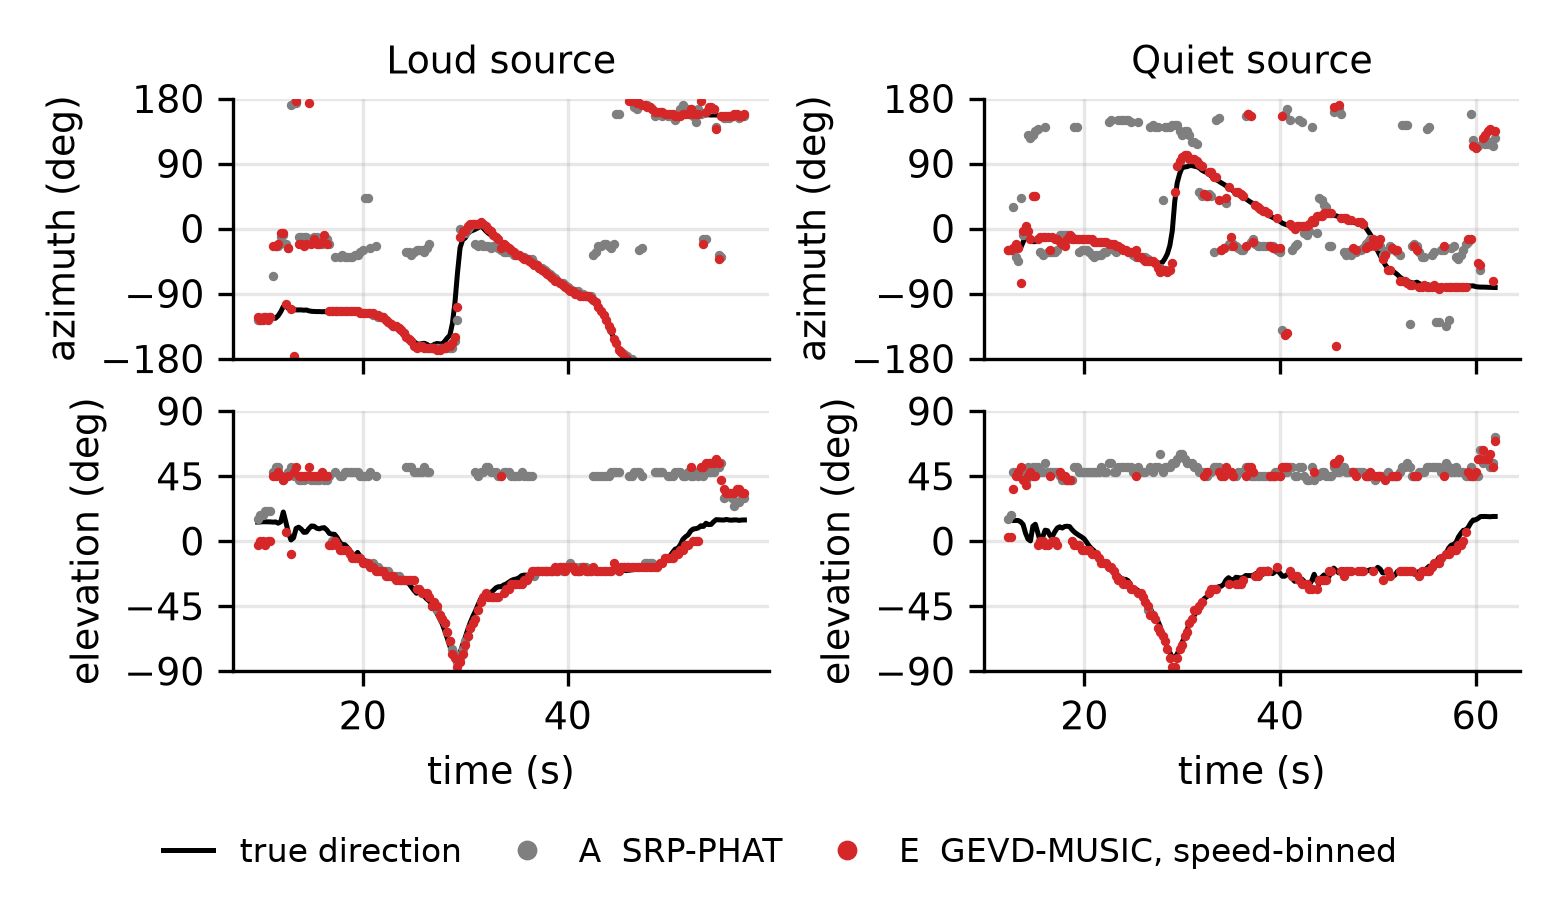
\includegraphics[width=0.82\textwidth]{fig/dregon_tracking.png}
\caption{True source direction (black) against the SRP-PHAT baseline (gray) and the speed-binned noise model (red) over two DREGON flights. The baseline locks onto the rotors at about $45$--$50^\circ$ elevation; the noise-model method follows the source through the maneuver.}
\label{fig:tracking}
\end{figure*}

\paragraph{Noise level.}
On clean recordings mixed with flight noise, all methods are accurate at 0 and $-5$\,dB.
At $-10$\,dB, D and E still localize 90\% of 48 trials within $10^\circ$, against 40--46\% for the others; at $-20$\,dB every method fails.
The noise model therefore buys about 5\,dB of operating range, but no method reaches the SNR at which distant calls for help would be heard.

\paragraph{Signal quality.}
Because a beamformer is linear, the target and the noise can be passed through it separately and the output SNR measured exactly.
Steering an MVDR beamformer (\cref{eq:mvdr}) with the learned covariance towards E's \emph{estimated} direction raises the SNR over a single microphone by a median of 9.7\,dB with speed-binned and 9.1\,dB with a single covariance, against 4.0\,dB for delay-and-sum, over 48 mixtures at $-10$\,dB input SNR.
\Cref{fig:snrfreq} shows that the gain is largest between 1 and 4\,kHz.

\begin{figure}[t]
\centering
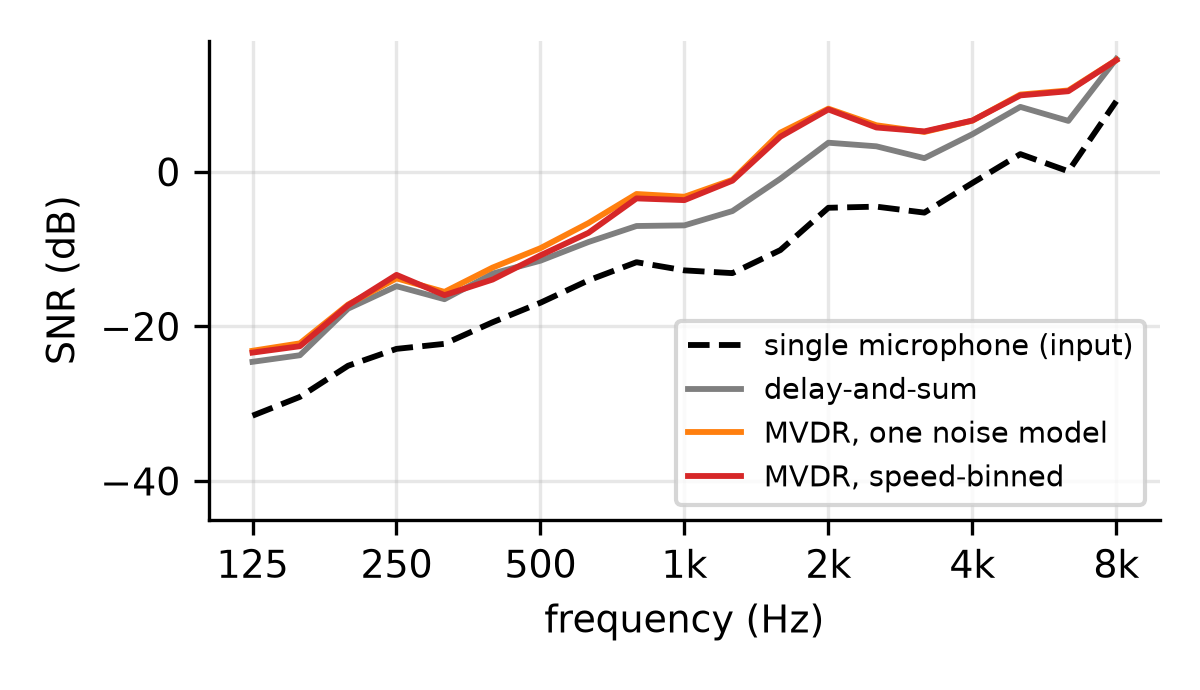
\includegraphics[width=\linewidth]{fig/dregon_snr_by_frequency.png}
\caption{SNR by third-octave band before (single microphone, dashed) and after beamforming towards the estimated direction, averaged over 48 mixtures at $-10$\,dB input SNR. A learned noise covariance (MVDR) roughly doubles the gain of plain delay-and-sum.}
\label{fig:snrfreq}
\end{figure}

\paragraph{Rotor tones and the IMU.}
Rotor tones are predictable from the motor log, but most of the noise energy on this drone is not on those tones.
The flight controller's IMU, sampled at about 1\,kHz, cannot observe vibration above 500\,Hz, which covers the lowest rotor harmonics (from about 140\,Hz) but not the band used for localization.

\subsection{Ego-noise across five drones}
\label{sec:case-drones}

A single drone cannot show whether these findings are general.
We therefore analyze noise-only recordings of four more quadrotors with 8-microphone arrays, released with the IEEE Signal Processing Cup 2019~\cite{deleforge2019spcup}: a DJI Phantom~4 Pro hovering outdoors at 2 and 10\,m, an MK Quadro~V3, an Intel Aero in manually controlled hover, and a quadrotor recorded at varying rotor speeds in an anechoic chamber (team AGH).
Of the other multichannel sets in that collection, two could no longer be downloaded, and one used a 16-microphone array whose published coordinates conflict with its photographs, so we did not use them.
Because the arrays differ, we use two measures that need no array geometry (\cref{fig:drones}).
The \emph{tonal share} is the share of 100--4000\,Hz noise energy in narrow spectral peaks, at least 6\,dB above a 300\,Hz running-median floor, computed on 1\,s chunks and averaged.
We define the \emph{learned rejection} to measure spatial structure.
It builds on the model of Wang and Cavallaro~\cite{wang2016earinthesky}, in which each rotor acts as one directional noise source and a diffuse part is added.
Because the microphones and motors are fixed to the frame, the acoustic mixing is stationary.
We learn the four strongest noise directions on the first half of a recording, one per rotor, and remove them from the second half with an orthogonal projection, as in the eigencanceler~\cite{haimovich1996eigencanceler}.
The learned rejection is the resulting drop in noise power, averaged over 300--4000\,Hz bins.
For the three arrays whose geometry was published, we compare it with a spherically diffuse noise field on the same array.

\begin{figure*}[t]
\centering
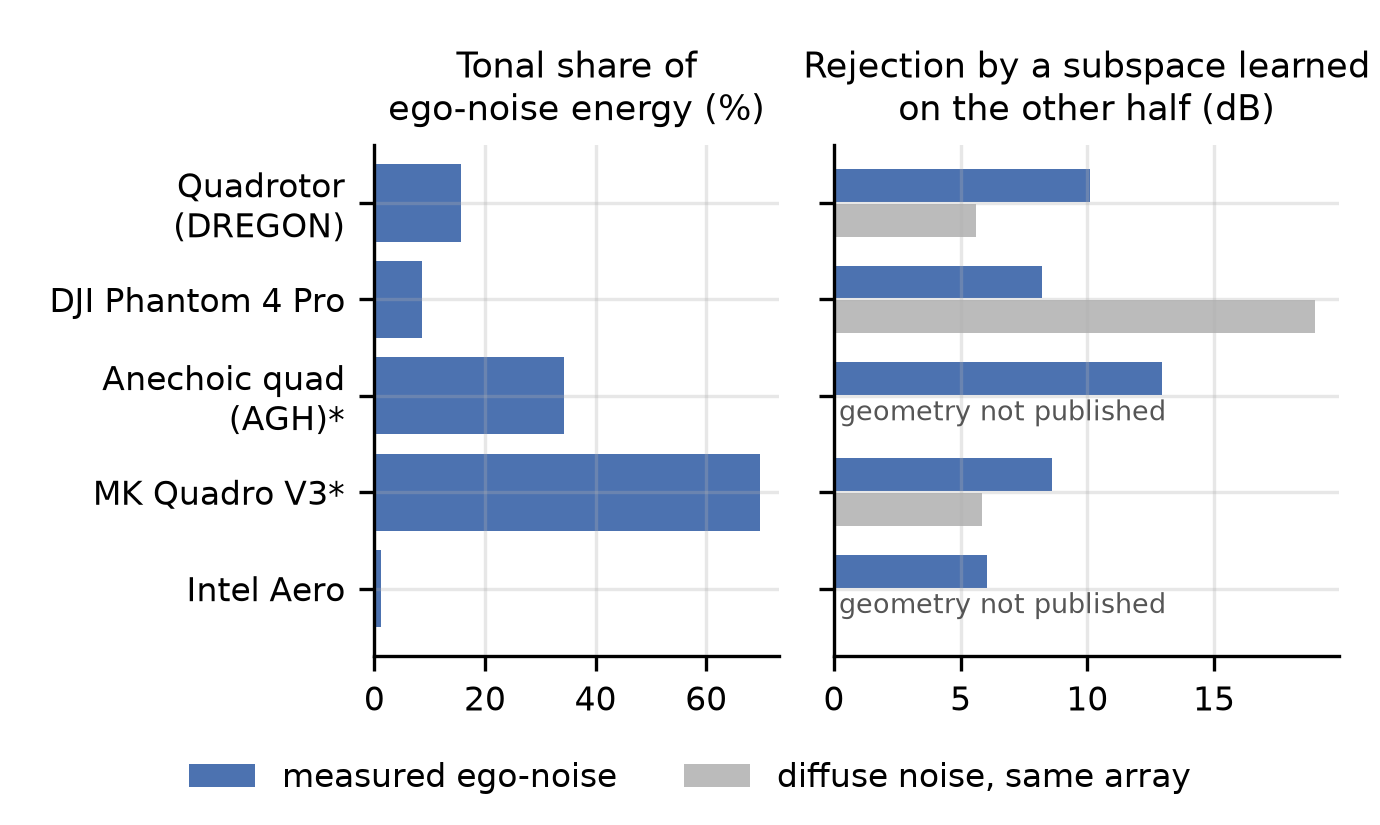
\includegraphics[width=0.68\textwidth]{fig/multidrone_egonoise.png}
\caption{Ego-noise of five quadrotors. Left: share of noise energy in rotor tones. Right: noise power removed from one half of a recording by a four-dimensional spatial subspace learned on the other half, against a diffuse noise field on the same array where the geometry is published. * represents a drone that was not flying during the recording. The MK Quadro~V3 was held about 0.5\,m above the floor. The AGH quadrotor stood still in an anechoic chamber.}
\label{fig:drones}
\end{figure*}

\paragraph{Results.}
Tonality differs by a factor of about 60 between drones: from 1\% of the noise energy (Intel Aero) through 16\% (DREGON) to 70\% (MK Quadro~V3).
However, the two highest values come from drones that were not in self-powered flight.
They are marked with an asterisk (*) in \cref{fig:drones}.
Among the three flying drones, the tonal share differs by a factor of about 13.
Masking or cancelling rotor tones is therefore valuable on some drones and nearly irrelevant on others.
A learned spatial subspace removes 6 to 13\,dB on every drone, and the model stays valid from one half of a recording to the other.
On the DREGON and MK Quadro~V3 arrays, with apertures of 17 and 15\,cm, it removes 4.5 and 2.7\,dB more than it would from diffuse noise, so the rotor noise is spatially more structured than background noise.
On the 6\,cm DJI Phantom array, however, a spatial model removes \emph{less} ego-noise than it would remove from diffuse noise (8.2 against 19.0\,dB).
This suggests that the noise is uncorrelated between the microphones.
Airflow over each microphone capsule may cause this.
Spatial models cannot remove such noise; larger apertures, flow shielding or single-channel suppression are needed instead.

\paragraph{Flight condition and tonality.}
In flight, the controller continually adjusts the rotor speeds.
This smears the rotor harmonics over each analysis window.
We measured the rotor-speed variation in each 1\,s window of the DREGON noise-only flight as the standard deviation of the logged speeds.
Windows with more variation have a lower tonal share (Spearman $\rho=-0.34$, $p=0.016$, 50 windows).
At the same mean rotor speed, their harmonic peaks are also lower (\cref{fig:jitter}).
Tonality measured on a drone that is not flying can therefore overstate the tonality in flight.

\begin{figure*}[t]
\centering
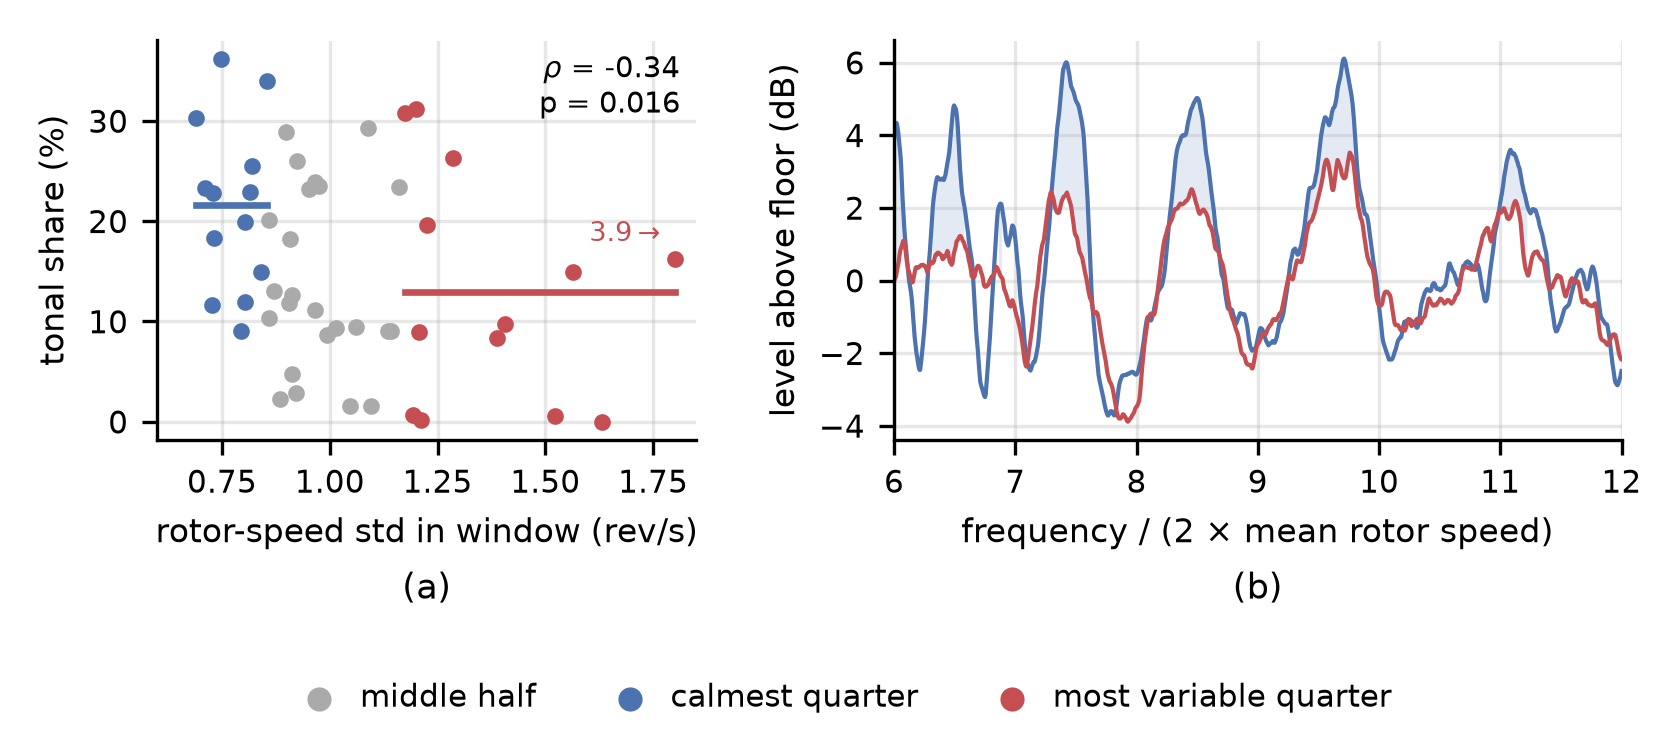
\includegraphics[width=0.78\textwidth]{fig/dregon_jitter_tonal.png}
\caption{Rotor-speed variation and tonal share in the DREGON noise-only flight (50 windows of 1\,s). (a) Tonal share against the standard deviation of the rotor speeds within each window. The standard deviation is averaged over the four rotors. Horizontal lines mark the mean of the calmest quarter (21.6\%) and of the most variable quarter (12.9\%). One window with 3.9\,rev/s is drawn at the edge. (b) Mean spectrum of these two quarters. Each window is aligned to its own mean rotor speed. Both quarters have the same mean speed (80.7 and 80.8\,rev/s). The harmonic peaks are lower in the variable windows (shaded).}
\label{fig:jitter}
\end{figure*}

\subsection{A robot-head array in a reverberant room (LOCATA)}
\label{sec:case-locata}

To test the localizers on a different platform and array, we use the robot-head array of the LOCATA development set~\cite{lollmann2018locata,evers2020locata}: a prototype NAO head with 12 microphones in a pseudo-spherical arrangement, recorded in a room with a reverberation time of about 0.5\,s, with optical tracking of the array and the sources and voice activity labels for every sample.
We use the three single-source tasks: a static loudspeaker with a static array (task~1), a moving talker with a static array (task~3), and a moving talker with a moving array (task~5).
The ground-truth direction is computed in the array's own frame from the tracked pose, so no alignment is fitted, and windows are scored when the source is active in at least 80\% of their samples (396 windows in total).
Methods B and E need motor speeds, which this platform lacks; method D learns its noise covariance from frames of the same recording in which the source is silent, at least 0.5\,s from any speech so that the reverberant tail does not leak in (or from all silent frames when fewer than 20 such frames exist).
The head has no running motors, so this study probes a regime without ego-noise.

\begin{table}[t]
\centering
\footnotesize
\setlength{\tabcolsep}{2.2pt}
\begin{tabular}{@{}lccc@{}}
\toprule
Method & Task 1 (34) & Task 3 (151) & Task 5 (211) \\
\midrule
A\; SRP-PHAT & 100\% / $4.8^\circ$ & \textbf{91.4\%} / $\mathbf{2.8^\circ}$ & \textbf{99.1\%} / $\mathbf{2.8^\circ}$ \\
C\; MUSIC & 100\% / $3.1^\circ$ & 86.1\% / $3.2^\circ$ & 95.7\% / $2.8^\circ$ \\
D\; GEVD, 0.5\,s guard & 100\% / $3.2^\circ$ & 69.5\% / $5.4^\circ$ & 68.2\% / $4.0^\circ$ \\
D\; GEVD, no guard & 100\% / $\mathbf{2.8^\circ}$ & 58.3\% / $8.0^\circ$ & 81.0\% / $4.6^\circ$ \\
\bottomrule
\end{tabular}
\caption{Localization with the LOCATA robot-head array: share of windows within $10^\circ$ / median angular error. Window counts in parentheses. Task 1: static loudspeaker and array; task 3: moving talker; task 5: moving talker and moving array.}
\label{tab:locata}
\end{table}

\paragraph{Results.}
\Cref{tab:locata} shows that the classical localizers are accurate on this array: SRP-PHAT places 91 to 100\% of windows within $10^\circ$, with median errors of 2.8 to $4.8^\circ$, also when both the talker and the array move.
The noise model does not help here; with moving talkers it lowers the share within $10^\circ$ by 18 to 33 points relative to SRP-PHAT, whether or not the reverberant tail is excluded.
The diagnostics explain why.
The SNR at the array is high, 16 to 25\,dB across recordings, and the background noise is close to diffuse: 75 to 89\% of its energy lies in the four strongest spatial components, against 79\% for a diffuse field on the same array.
There is little structured noise to remove, so whitening with a covariance estimated from a few hundred frames of changing background noise mainly distorts the spatial spectrum.

\subsection{What the case studies show}

Taken together, the three studies support a qualified version of the argument of \cref{sec:egonoise}.
\emph{(i)} When ego-noise dominates and is spatially structured, an explicit noise model is the largest single gain: on DREGON it raised in-flight accuracy within $10^\circ$ from 18\% to 70\%, and spatial noise models removed 6 to 13\,dB of ego-noise on all five drones.
\emph{(ii)} State information adds most when the target is weak: motor-speed-binned models gained 17 points over a single model on the quiet-source flight.
\emph{(iii)} The value of tone-based methods depends on the drone and on whether it is flying. Tonality ranged from 1\% to 70\% of the ego-noise energy, and rotor-speed variation in flight lowered it.
\emph{(iv)} A noise model is not free: when the SNR is high and the background close to diffuse, as on the robot head, it costs accuracy, so a system should decide from the measured noise conditions whether to apply it.
\emph{(v)} Array aperture and airflow limit what any spatial model can do, as the 6\,cm array showed.
All methods in these studies are established; the contribution is the controlled, reproducible comparison across platforms.
